\documentclass[times,t]{beamer}
\usepackage{amssymb}
\usepackage{amsmath}
\usepackage{amsfonts}
\usepackage{lmodern} 
\input{sym.tex}
\setbeamertemplate{navigation symbols}{}

\title{ECE 417/598: Plane to points and DLT}
\author{Vikas Dhiman.  }
\date{March 21, 2022}
\DeclareMathOperator{\diag}{diag}
\begin{document}

\newcommand{\ubfu}{\underline{\bfu}}
\begin{frame}
  \titlepage
  \end{frame}
\begin{frame}
  \includegraphics[width=\linewidth]{media/lane-from-points.pdf}
  \begin{align*}
    \ubfu_1 &= [100, 98, 1]^\top\\
    \ubfu_2 &= [105, 95, 1]^\top\\
    \ubfu_3 &= [107, 90, 1]^\top\\
    \ubfu_4 &= [110, 85, 1]^\top
    \end{align*}
    Find  the line $\bfl$ such that it is the ``closest line'' passing through
    $\bfu_1, \dots, \bfu_4$.
\end{frame}

\begin{frame}
  \begin{align*}
  A = \begin{bmatrix}\bfu_1^\top  \\
    \bfu_2^\top \\
    \bfu_3^\top \\
    \bfu_4^\top
  \end{bmatrix}
  \end{align*}
  We want to solve for $\bfl$ such that
  \begin{align*}
    A \bfl = 0
  \end{align*}
\end{frame}

\begin{frame}{Singular Value  Decomposition (SVD)}
  \begin{align*}
    A  &=   U  \begin{bmatrix}\Sigma   &  0  \\   0  &  0 \end{bmatrix} V^\top
  \end{align*}
  \begin{align*}
    A^\top A &= V \Sigma^2  V^{-1}
  \end{align*}
  \begin{align*}
    A^\top A \bfv_i  &= \lambda_i \bfv_i & \lambda_i = \sigma_i^2, \Sigma = \diag([\sigma_1, \dots, \sigma_r])\\
  \end{align*}
  \begin{align*}
    \bfu_i   &=  \frac{A\bfv_i}{\sigma_i}
    \end{align*}
    \begin{align*}
      U = \begin{bmatrix}
        \bfu_1 & \bfu_2 & \dots & \bfu_m
      \end{bmatrix}
    \end{align*}
\end{frame}

\begin{frame}
  If $A \in \bbR^{m \times n}$ and the rank of $A$ is $r$, then
  \begin{align*}
    A  &=   \begin{bmatrix}U_{m\times r} & U_{m \times (m-r),\perp}\end{bmatrix}  \begin{bmatrix}\Sigma_{r \times r}   &  0_{r \times (n-r)}  \\   0_{(m-r)\times r}  &  0_{(m-r)\times (n-r)} \end{bmatrix} \begin{bmatrix} V_{n \times r}^\top  \\ V_{n \times (n-r),\perp}^\top \end{bmatrix}
    \\
    A &= U_{m \times r} \Sigma_{r \times r} V_{n \times r}^\top + 0 * U_{m \times (m-r),\perp} V_{n \times (n-r),\perp}^\top
  \end{align*}
\end{frame}

\begin{frame}

  \begin{center}
  \includegraphics[width=0.5\linewidth]{./media/four-fundamental-subspaces.png}
  \end{center}
  \begin{align*}
    \calN(A) &= V_{n\times (n-r),\perp}
               \\
    \calR(A) &= U_{m\times r}
    \\
    \calN(A^\top) &= U_{m\times (m-r),\perp}
    \\
    \calR(A^\top) &= V_{n\times r}
    \end{align*}
\end{frame}


\begin{frame}
  \includegraphics[width=\linewidth]{media/lane-from-points.pdf}

  We want to solve for $\bfl$ such that
  \begin{align*}
    A \bfl = 0
  \end{align*}

  $A$ is $m \times 3$ and has rank $2$. Solution
  \begin{align*}
    U \Sigma V^\top = A
    \\
    V = [\bfv_1, \bfv_2, \bfv_3]
    \\
    \bfl = \bfv_3
  \end{align*}
\end{frame}
\newcommand{\ubfx}{\underline{\bfx}}
\begin{frame}
  \includegraphics[width=\linewidth]{media/plane-from-points.pdf}

  {\small
  \begin{align*}
  \ubfx_1 &= [-2.3, 1.04, 3.2, 1]^\top & 
  \ubfx_2 &= [-2.2, 1.02, 2.2, 1]^\top\\
  \ubfx_3 &= [-2.1, 1.01, 1.2, 1]^\top & 
  \ubfx_4 &= [2.1, 1.04, 1.2, 1]^\top \\
  \ubfx_5 &= [2.2, 1.03, 3.2, 1]^\top  &
  \ubfx_6 &= [2.3, 1.01, 4.2, 1]^\top
  \end{align*}
  }
  Find the equation of plane $\bfp = [p_1, p_2, p_3, p_4]^\top$ such  all points
  lie on the plane.
\end{frame}

\begin{frame}

%   {\small
%     \begin{align*}
%       \ubfx_1^\top \bfp &= 0  &
%                                 \ubfx_2^\top \bfp &= 0 \\
%       \ubfx_3^\top \bfp &= 0  &
%                                 \ubfx_4^\top \bfp &= 0 \\
%       \ubfx_5^\top \bfp &= 0  &
%                                 \ubfx_6^\top \bfp &= 0 \\
%     \end{align*}
%   }
%   Construct $A \in \bbR^{6 \times 4}$ with the points
%   \begin{align*}
%     A = \begin{bmatrix}
%       \ubfx_1^\top \\ \ubfx_2^\top \\ \ubfx_3^\top \\ \ubfx_4^\top \\ \ubfx_5^\top \\ \ubfx_6^\top
%       \end{bmatrix}
%     \end{align*}
% 
% We want to solve for $\bfp$ such that
% \begin{align*}
%   A \bfp = 0
% \end{align*}

\end{frame}
\begin{frame}
%  $A$ is $m \times 4$ and has rank $3$. Solution
%  \begin{align*}
%    U \Sigma V^\top = A
%    \\
%    V = [\bfv_1, \bfv_2, \bfv_3, \bfv_4]
%    \\
%    \bfp = \bfv_4
%  \end{align*}
\end{frame}

\begin{frame}
  \includegraphics[width=\linewidth]{media/lane-from-points.pdf}
  \begin{align*}
    \ubfx_1 &= [100, 98, 45,1]^\top\\
    \ubfx_2 &= [105, 95, 46, 1]^\top\\
    \ubfx_3 &= [107, 90, 47,1]^\top\\
    \ubfx_4 &= [110, 85, 43,1]^\top
  \end{align*}
  Find  the 3D line such that it is the ``closest line'' passing through
  $\bfx_1, \dots, \bfx_4 \in \bfP^3$.
\end{frame}

\begin{frame}
\end{frame}

\begin{frame}{Implicit and parameteric equations of lines and plane} 

\end{frame}

\begin{frame}{Homography}
  \includegraphics[width=\linewidth]{media/homography-maps-a-line-to-a-line.png}
\end{frame}

\begin{frame}{Examples  of  Homography}
  \includegraphics[width=\linewidth]{media/examples-of-homography.png}
\end{frame}

\begin{frame}
  \includegraphics[width=0.60\linewidth]{media/audi top view camera.jpg}
\end{frame}

\begin{frame}{Computing Homography}
  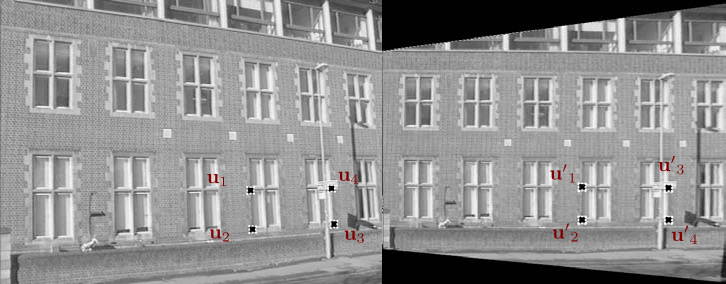
\includegraphics[width=\linewidth]{media/removing-perspective-distortion.png.pdf}
  \begin{align*}
    \ubfu_1 &= [100, 98, 1]^\top&
    \ubfu_2 &= [102, 95, 1]^\top\\
    \ubfu_3 &= [107, 90, 1]^\top&
    \ubfu_4 &= [110, 85, 1]^\top \\
    \ubfu'_1 &= [100, 98, 1]^\top&
    \ubfu'_2 &= [102, 95, 1]^\top\\
    \ubfu'_3 &= [107, 98, 1]^\top&
    \ubfu'_4 &= [110, 85, 1]^\top
  \end{align*}
  Find $H$ such that $\ubfu' = H\ubfu$ for any point on one image to another image.
\end{frame}

\begin{frame}{2D homography}
  Given a set of points $\ubfu_i \in \bbP^2$ and a corresponding set of
  points $\ubfu'_i \in \bbP^2$, compute the projective transformation that takes each
  $\ubfu_i$ to $\ubfu'_i$ . In a practical situation, the points $\ubfu_i$ and   $\ubfu'_i$  are points in two images
  (or the same image), each image being considered as a projective plane  $\bbP^2$.
\end{frame}

\begin{frame}{Solving for Homography }
\end{frame}


\begin{frame}{3D  to  2D camera projection matrix estimation}
  Given a set of points $\bfX_i$ in 3D space, and a set
  of corresponding points $\bfx_i$ in an image, find the 3D to 2D projective
  $\bfP$ mapping
  that maps $\bfX_i$ to $\bfx_i  =  \bfP\bfX_i$.
\end{frame}

\end{document}